\documentclass[onlymath]{beamer}
% \documentclass[onlymath,handout]{beamer}

% Macros used by all lectures, but not necessarily by excercises

%%% General setup and dependencies:

% \usetheme[ddcfooter,nosectionnum]{tud}
\usetheme[nosectionnum,pagenum,noheader]{tud}
% \usetheme[nosectionnum,pagenum]{tud}

% Increase body font size to a sane level:
\let\origframetitle\frametitle
% \renewcommand{\frametitle}[1]{\origframetitle{#1}\normalsize}
\renewcommand{\frametitle}[1]{\origframetitle{#1}\fontsize{10pt}{13.2}\selectfont}
\setbeamerfont{itemize/enumerate subbody}{size=\small} % tud defaults to scriptsize!
\setbeamerfont{itemize/enumerate subsubbody}{size=\small}
% \setbeamerfont{normal text}{size=\small}
% \setbeamerfont{itemize body}{size=\small}

\renewcommand{\emph}[1]{\textbf{#1}}

\def\arraystretch{1.3}% Make tables even less cramped vertically

\usepackage[ngerman]{babel}
\usepackage[utf8]{inputenc}
\usepackage[T1]{fontenc}

%\usepackage{graphicx}
\usepackage[export]{adjustbox} % loads graphicx
\usepackage{import}
\usepackage{stmaryrd}
\usepackage[normalem]{ulem} % sout command
% \usepackage{times}
\usepackage{txfonts}
\usepackage{array}

% \usepackage[perpage]{footmisc} % reset footnote counter on each page -- fails with beamer (footnotes gone)
\usepackage{perpage}  % reset footnote counter on each page
\MakePerPage{footnote}

\usepackage{tikz}
\usetikzlibrary{arrows,positioning,decorations.pathreplacing}
% Inspired by http://www.texample.net/tikz/examples/hand-drawn-lines/
\usetikzlibrary{decorations.pathmorphing}
\pgfdeclaredecoration{penciline}{initial}{
    \state{initial}[width=+\pgfdecoratedinputsegmentremainingdistance,
    auto corner on length=1mm,]{
        \pgfpathcurveto%
        {% From
            \pgfqpoint{\pgfdecoratedinputsegmentremainingdistance}
                      {\pgfdecorationsegmentamplitude}
        }
        {%  Control 1
        \pgfmathrand
        \pgfpointadd{\pgfqpoint{\pgfdecoratedinputsegmentremainingdistance}{0pt}}
                    {\pgfqpoint{-\pgfdecorationsegmentaspect
                     \pgfdecoratedinputsegmentremainingdistance}%
                               {\pgfmathresult\pgfdecorationsegmentamplitude}
                    }
        }
        {%TO
        \pgfpointadd{\pgfpointdecoratedinputsegmentlast}{\pgfpoint{1pt}{1pt}}
        }
    }
    \state{final}{}
}
\tikzset{handdrawn/.style={decorate,decoration=penciline}}
\tikzset{every shadow/.style={fill=none,shadow xshift=0pt,shadow yshift=0pt}}
% \tikzset{module/.append style={top color=\col,bottom color=\col}}

% Use to make Tikz attributes with Beamer overlays
% http://tex.stackexchange.com/a/6155
\tikzset{onslide/.code args={<#1>#2}{%
  \only<#1| handout:0>{\pgfkeysalso{#2}}
}}
\tikzset{onslideprint/.code args={<#1>#2}{%
  \only<#1>{\pgfkeysalso{#2}}
}}

%%% Title -- always set this first

\newcommand{\defineTitle}[3]{
	\newcommand{\lectureindex}{#1}
	\title{Theoretische Informatik und Logik}
	\subtitle{\href{\lectureurl}{#1. Vorlesung: #2}}
	\author{\href{https://iccl.inf.tu-dresden.de/web/Markus_Kr\%C3\%B6tzsch}{Markus Kr\"{o}tzsch}\\[1ex]Lehrstuhl Wissensbasierte Systeme}
	\date{#3}
	\datecity{TU Dresden}
% 	\institute{CC-By 3.0, sofern keine anderslautenden Bildrechte angegeben sind}
}

%%% Table of contents:

\RequirePackage{ifthen}

\newcommand{\highlight}[2]{%
	\ifthenelse{\equal{#1}{\lectureindex}}{\alert{#2}}{#2}%
}

\def\myspace{-0.7ex}
\newcommand{\printtoc}{
\begin{tabular}{r@{$\quad$}l}
\highlight{1}{1.} & \highlight{1}{Willkommen/Einleitung formale Sprachen}\\[\myspace]
\highlight{2}{2.} & \highlight{2}{Grammatiken und die Chomsky-Hierarchie}\\[\myspace]
\highlight{3}{3.} & \highlight{3}{Endliche Automaten}\\[\myspace]
\highlight{4}{4.} & \highlight{4}{Complexity of FO query answering}\\[\myspace]
\highlight{5}{5.} & \highlight{5}{Conjunctive queries}\\[\myspace]
\highlight{6}{6.} & \highlight{6}{Tree-like conjunctive queries}\\[\myspace]
\highlight{7}{7.} & \highlight{7}{Query optimisation}\\[\myspace]
\highlight{8}{8.} & \highlight{8}{Conjunctive Query Optimisation / First-Order~Expressiveness}\\[\myspace]
\highlight{9}{9.} & \highlight{9}{First-Order~Expressiveness / Introduction to Datalog}\\[\myspace]
\highlight{10}{10.} & \highlight{10}{Expressive Power and Complexity of Datalog}\\[\myspace]
\highlight{11}{11.} & \highlight{11}{Optimisation and Evaluation of Datalog}\\[\myspace]
\highlight{12}{12.} & \highlight{12}{Evaluation of Datalog (2)}\\[\myspace]
\highlight{13}{13.} & \highlight{13}{Graph Databases and Path Queries}\\[\myspace]
\highlight{14}{14.} & \highlight{14}{Outlook: database theory in practice}
\end{tabular}
}

\newcommand{\overviewslide}{%
\begin{frame}\frametitle{Overview}
\printtoc
\medskip

Siehe \href{\lectureurl}{course homepage [$\Rightarrow$ link]} for more information and materials
\end{frame}
}

%%% Colours:
\usepackage{xcolor,colortbl}
\definecolor{redhighlights}{HTML}{FFAA66}
\definecolor{lightblue}{HTML}{55AAFF}
\definecolor{lightred}{HTML}{FF5522}
\definecolor{lightpurple}{HTML}{DD77BB}
\definecolor{lightgreen}{HTML}{55FF55}
\definecolor{darkred}{HTML}{CC4411}
\definecolor{darkblue}{HTML}{176FC0}%{1133AA}
\definecolor{nightblue}{HTML}{2010A0}%{1133AA}
\definecolor{alert}{HTML}{176FC0}
\definecolor{darkgreen}{HTML}{36AB14}
\definecolor{strongyellow}{HTML}{FFE219}
\definecolor{devilscss}{HTML}{666666}

\newcommand{\redalert}[1]{\textcolor{darkred}{#1}}

%%% Slide layout commands:

\newcommand{\sectionSlide}[1]{
\frame{\begin{center}
\LARGE
#1
\end{center}}
}
\newcommand{\sectionSlideNoHandout}[1]{
\frame<handout:0>{\begin{center}
\LARGE
#1
\end{center}}
}

\newcommand{\mydualbox}[3]{%
 \begin{minipage}[t]{#1}
 \begin{beamerboxesrounded}[upper=block title,lower=block body,shadow=true]%
    {\centering\usebeamerfont*{block title}#2}%
    \raggedright%
    \usebeamerfont{block body}
%     \small
    #3%
  \end{beamerboxesrounded}
  \end{minipage}
}
%
\newcommand{\myheaderbox}[2]{%
 \begin{minipage}[t]{#1}
 \begin{beamerboxesrounded}[upper=block title,lower=block title,shadow=true]%
    {\centering\usebeamerfont*{block title}\rule{0pt}{2.6ex} #2}%
  \end{beamerboxesrounded}
  \end{minipage}
}

\newcommand{\mycontentbox}[2]{%
 \begin{minipage}[t]{#1}%
 \begin{beamerboxesrounded}[upper=block body,lower=block body,shadow=true]%
    {\centering\usebeamerfont*{block body}\rule{0pt}{2.6ex}#2}%
  \end{beamerboxesrounded}
  \end{minipage}
}

\newcommand{\mylcontentbox}[2]{%
 \begin{minipage}[t]{#1}%
 \begin{beamerboxesrounded}[upper=block body,lower=block body,shadow=true]%
    {\flushleft\usebeamerfont*{block body}\rule{0pt}{2.6ex}#2}%
  \end{beamerboxesrounded}
  \end{minipage}
}

% label=180:{\rotatebox{90}{{\footnotesize\textcolor{darkgreen}{Beispiel}}}}
% \hspace{-8mm}\ghost{\raisebox{-7mm}{\rotatebox{90}{{\footnotesize\textcolor{darkgreen}{Beispiel}}}}}\hspace{8mm}
\newcommand{\examplebox}[1]{%
	\begin{tikzpicture}[decoration=penciline, decorate]
		\pgfmathsetseed{1235}
		\node (n1) [decorate,draw=darkgreen, fill=darkgreen!10,thick,align=left,text width=\linewidth, inner ysep=2mm, inner xsep=2mm] at (0,0) {#1};
% 		\node (n2) [align=left,text width=\linewidth,inner sep=0mm] at (n1.92) {{\footnotesize\raisebox{3mm}{\textcolor{darkgreen}{Beispiel}}}};
% 		\node (n2) [decorate,draw=darkgreen, fill=darkgreen!10,thick, align=left,text width=\linewidth,inner sep=2mm] at (n1.90) {{\footnotesize\raisebox{0mm}{\textcolor{darkgreen}{Beispiel}}}};
	\end{tikzpicture}%
}%

\newcommand{\codebox}[1]{%
	\begin{tikzpicture}[decoration=penciline, decorate]
		\pgfmathsetseed{1236}
		\node (n1) [decorate,draw=strongyellow, fill=strongyellow!10,thick,align=left,text width=\linewidth, inner ysep=2mm, inner xsep=2mm] at (0,0) {#1};
	\end{tikzpicture}%
}%

\newcommand{\defbox}[1]{%
	\begin{tikzpicture}[decoration=penciline, decorate]
		\pgfmathsetseed{1237}
		\node (n1) [decorate,draw=darkred, fill=darkred!10,thick,align=left,text width=\linewidth, inner ysep=2mm, inner xsep=2mm] at (0,0) {#1};
	\end{tikzpicture}%
}%

\newcommand{\theobox}[1]{%
	\begin{tikzpicture}[decoration=penciline, decorate]
		\pgfmathsetseed{1240}
		\node (n1) [decorate,draw=darkblue, fill=darkblue!10,thick,align=left,text width=\linewidth, inner ysep=2mm, inner xsep=2mm] at (0,0) {#1};
	\end{tikzpicture}%
}%

\newcommand{\anybox}[2]{%
	\begin{tikzpicture}[decoration=penciline, decorate]
		\pgfmathsetseed{1240}
		\node (n1) [decorate,draw=#1, fill=#1!10,thick,align=left,text width=\linewidth, inner ysep=2mm, inner xsep=2mm] at (0,0) {#2};
	\end{tikzpicture}%
}%


\newsavebox{\mybox}%
\newcommand{\doodlebox}[2]{%
\sbox{\mybox}{#2}%
	\begin{tikzpicture}[decoration=penciline, decorate]
		\pgfmathsetseed{1238}
		\node (n1) [decorate,draw=#1, fill=#1!10,thick,align=left,inner sep=1mm] at (0,0) {\usebox{\mybox}};
	\end{tikzpicture}%
}%


\defineTitle{11}{NL und PSpace}{19. Mai 2017}

\begin{document}

\maketitle

\begin{frame}\frametitle{\Scomplclass{NP}-vollständige Probleme}

\Scomplclass{NP}-vollständige Probleme\\ = Probleme, die mindestens so schwer
sind, wie alle anderen Probleme in \Scomplclass{NP}\\
= die schwersten Probleme in NP.
\bigskip

\emph{Alles oder nichts:}\\
Entweder sind alle NP-vollständigen Probleme in P\\
oder kein einziges NP-vollständiges Problem ist in P
\bigskip\pause

\alert{Ladner:} "`Alle glauben P${}\neq{}$NP. Dann gibt es aber auch 
beliebig viele Probleme in NP, die nicht NP-vollständig sind und dennoch nicht in P liegen."'
\\
\medskip
\emph{Anders gesagt:} Neben den "`schwersten"' Problemen in NP gibt es dann auch noch viele "`mittelschwere"', welche dennoch nicht in P liegen. Bisher wissen wir nicht, welche das
sind.

\end{frame}

\begin{frame}\frametitle{Leichte NP-vollständige Probleme}

Pseudopolynomielle Probleme sind polynomiell in der Größe von
Eingabe und gegebenen Zahlenbeträgen.
\bigskip

Das macht sie in der Praxis oft eher einfach.
\bigskip

\examplebox{
Beispiel: Das Rucksackproblem ist nur dann NP-vollständig,
wenn die Gewichte der Gegenstände über-polynomiell wachsen dürfen. Ein Problem mit
so schweren Gegenständen ist aber nur dann interessant, wenn auch der Rucksack
eine sehr große Kapazität hat. Alternativ könnte man mit sehr hoher Genauigkeit wiegen.
}

\end{frame}

\sectionSlide{NL}

\begin{frame}\frametitle{Die Macht des Speichers}

Selbst innerhalb kleiner Speichergrenzen ist sehr viel machbar:\pause
\begin{itemize}
\item \Slang{SAT} ist mit linearem Speicher lösbar:\\
Wir iterieren durch alle Wahrheitswertbelegungen (jeweils linear groß) und
testen jeweils, ob die Formel erfüllt ist (logarithmischer Speicher für ein paar Pointer und Zwischenergebnisse)\pause
\item Linearer Speicher genügt zur Erkennung kontextsensitiver Sprachen (durch linear beschränkte Automaten, LBA)\pause
\item Jedes NP-vollständige Problem ist in polynomiellen Speicher lösbar:\\
Wir iterieren durch alle polynomiellen Zertifikate und simulieren einen polynomiellen
Verifikator auf ihnen
\end{itemize}

$\leadsto$ sehr kleine Speichergrenzen sind sinnvoll

\end{frame}

\begin{frame}\frametitle{Erinnerung: L}

\emph{LogSpace (L):} Sprachen die man mit sehr wenig Arbeitsspeicher erkennen kann
\bigskip

\alert{Wesentliche Datentypen:} 
\begin{itemize}
\item Zähler, Maximalwert polynomiell beschränkt
\item Pointer auf (read-only) Eingabeband
\end{itemize}
{\tiny Jeweils fest deklariert, d.h. ihre Anzahl hängt nicht von der Eingabe ab

}
\bigskip

\alert{Wesentliche Programmierfeatures:}
\begin{itemize}
\item Initialisiere Pointer oder Zähler auf festen Wert
\item Inkrementiere/dekrementiere Pointer oder Zähler
\item Vergleiche Speicherinhalte von zwei Pointern oder zwei Zählern (und führe je nach Ergebnis anderen Code aus)
\end{itemize}
\bigskip

\alert{Optionaler Ausgabestrom:} Write-only, write once 

\end{frame}

\begin{frame}\frametitle{NLogSpace}

\alert{Nichtdeterministische TM mit logarithmischem Speicher:}
\[
\Scomplclass{NL} = \Scomplclass{NLogSpace} = \Scomplclass{NSpace}(\log n)
\]

\alert{Alternativ:}\\
"`Probleme, deren Lösung in L verifiziert werden kann"'
\bigskip

\begin{itemize}
\item Gleiche Programmierfeatures wie in L
\item Aber nichtdeterministische Operationen möglich,\\ z.B. setze Pointer auf eine zufällige Eingabeposition
\end{itemize}

\end{frame}

\begin{frame}\frametitle{Beispiel: Erreichbarkeit}

\defbox{Das Problem der (\Slang{s-t-})\Slang{Erreichbarkeit} in gerichteten Graphen
lautet wie folgt:\\[1ex]
\emph{Gegeben:} gerichteter Graph $G$ mit Knoten $s$ und $t$\\
\emph{Frage:} Gibt es in $G$ einen gerichteten Pfad von $s$ nach $t$?
}\bigskip\pause

\theobox{Satz:
\Slang{Erreichbarkeit} in gerichteten Graphen liegt in NL.}\pause

\emph{Beweis (Algorithmus):}
\begin{itemize}
\item Wir verweden einen Pointer $p$ auf einen Knoten (in der Eingabe) und einen Zähler $z$
\item Initialisiere $*p=s$ und $z=1$
\item Schleife:
\begin{itemize}
\item Falls $*p=t$ dann akzeptiere
\item Falls $z={}$Anzahl der Knoten in $G$ dann verwerfe
\item Andernfalls: inkrementiere $z$ und setze $p$ auf einen Nachfolger des aktuellen Knotens $*p$ (nichtdet.)\qed
\end{itemize}
\end{itemize}

\end{frame}

\begin{frame}\frametitle{NL-Vollständigkeit}

Man kann NL-Härte ähnlich wie für NP definieren:
\begin{itemize}
\item Statt polynomiellen Reduktionen verwendet man Logspace-Reduktionen
\item NL-hart: jedes Problem in NL ist darauf logspace-reduzierbar
\item NL-vollständig: in NL und NL-hart
\end{itemize}
Intuition: NL-vollständige Probleme sind die schwersten in NL
\bigskip\pause

\examplebox{Beispiel: \Slang{Erreichbarkeit} in gerichteten Graphen ist NL-vollständig.}\bigskip\pause

\examplebox{Beispiel: \Slang{Erreichbarkeit} in \redalert{un}gerichteten Graphen ist in NL aber nicht NL-hart: Das Problem liegt in L (Omer Reingold, 2005).}

\end{frame}

\begin{frame}\frametitle{L, NL und coNL}

\emph{Rückblick:} Savitch sagte uns, dass $\Scomplclass{NPSpace}=\Scomplclass{PSpace}$, also auch $\Scomplclass{NPSpace}=\Scomplclass{coNPSpace}$
\bigskip\pause

Für logarithmischen Speicher ergibt Savitchs Ergebnis aber lediglich: $\Scomplclass{NL}\subseteq\Scomplclass{NSpace}(\log^2 n)$
$\leadsto$ daraus folgt nicht $\Scomplclass{NL}\subseteq\Scomplclass{L}$!
\bigskip\pause

Man weiß dennoch:\bigskip

\theobox{Satz (Immerman 1987, Szelepcs\'enyi 1987): $\Scomplclass{NL}=\Scomplclass{coNL}$.}\pause\medskip

\examplebox{Beispiel: Nichterreichbarkeit in gerichteten Graphen kann in NL entschieden werden. Betrachtet man den NL-Algorithmus für Erreichbarkeit, dann ist das zunächst überraschend \ldots}
\bigskip

{\tiny
(Eng verwandtes Resultat: kontextsensitive Sprachen sind unter Komplement abgeschlossen)

}

\end{frame}

\sectionSlide{PSpace}

\begin{frame}\frametitle{Noch schwerere Probleme?}

\emph{Beobachtung:} Bisher waren alle entscheidbaren schweren Probleme der Vorlesung
auch in NP, d.h. ihre Lösung war leicht verifizierbar:

\begin{itemize}
\item \alert{Erfüllbarkeit}, \alert{Hamiltonpfad}, \alert{Clique}, \alert{Rucksack}: NP-vollständige Probleme mit polynomiellen Verifikatoren
\item \alert{Faktorisierung}: in $\Scomplclass{NP}\cap\Scomplclass{coNP}$
\item \alert{Erreichbarkeit in Graphen}: in NP (Zertifikat ist Pfad); sogar in P (z.B. Breitensuche)
\end{itemize}

Gibt es überhaupt noch schwerere entscheidbare Probleme?

\end{frame}

\begin{frame}\frametitle{Beispiel: Schachrätsel}

~\hfill
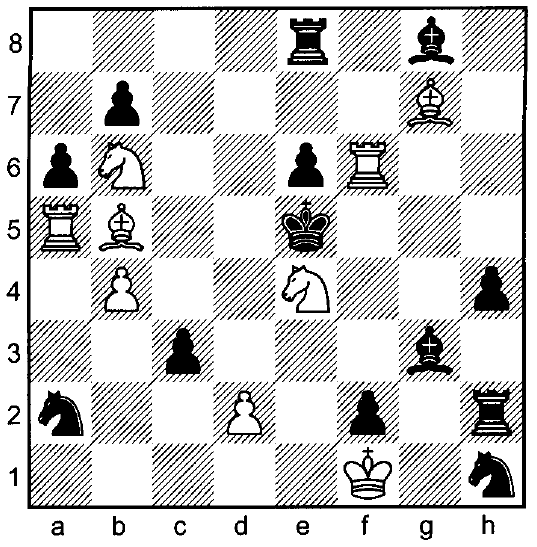
\includegraphics[height=6.5cm]{images/mate-3}
\hfill~

\narrowcentering{
Matt in drei Zügen; Weiß ist am Zug
}

\end{frame}

\begin{frame}\frametitle{Beispiel: Schachrätsel}

~\hfill
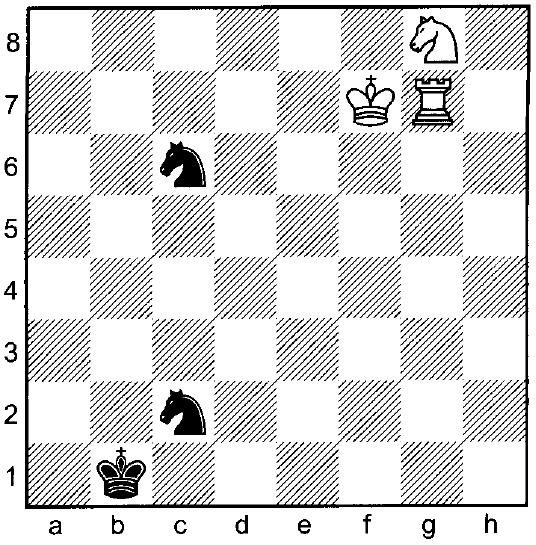
\includegraphics[height=6.5cm]{images/mate-262}
\hfill~

\narrowcentering{
Matt in 262 Zügen; Weiß ist am Zug
}

\end{frame}

\begin{frame}\frametitle{Rückblick Aussagenlogik}

\anybox{strongyellow}{\emph{Rückblick Aussagenlogik}\\[1ex]
%
\begin{itemize}
\item Aussagenlogische Formeln basieren auf \alert{Atomen} (Propositionen, Variablen)
\item Atome werden mit \alert{Junktoren} verknüpft: $\neg$, $\wedge$, $\vee$, $\to$\\ (wir setzen immer Klammern zwischen verschiedene binären Junktoren)
\item Wir erlauben außerdem die nullstelligen Operatoren $\top$ (wahr) und $\bot$ (falsch)
\item \alert{Belegungen} ordnen Atomen \alert{Wahrheitswerte} \mytrue{} oder \myfalse{} zu
\end{itemize}
}\pause

\begin{itemize}
\item \Slang{SAT}: Gegeben eine aussagenlogische Formel $\varphi$, \alert{existiert} eine Belegung der Atome in $\varphi$, für die $\varphi$ wahr wird?\pause
%
\item \Slang{Tautologie}: Gegeben eine aussagenlogische Formel $\varphi$, wird $\varphi$ \alert{für alle} Belegungen der Atome in $\varphi$ wahr?
\end{itemize}\pause
$\leadsto$
Existentielle und universelle Quantoren über Wahrheitswerte
\bigskip

\end{frame}


\begin{frame}\frametitle{Ein Problem in PSpace}

Ein Beispiel für ein erstes typisches PSpace-Problem ergibt sich, wenn man \Slang{SAT} und \Slang{Tautologie} verallgemeinert:\bigskip

\defbox{
Eine \redalert{Quantifizierte Boolsche Formel} (QBF) ist eine logische Formel der folgenden Form:
%
\[\quantor_1 p_1. \quantor_2 p_2. \cdots \quantor_\ell p_\ell.F[p_1,\ldots,p_\ell]\]
%
mit $i\geq 0$, $\quantor_i\in\{\exists,\forall\}$ Quantoren, $p_i$ aussagenlogischen Atomen (Variablen) und $F$ einer aussagenlogischen Formel mit Atomen $p_1,\ldots,p_\ell$.
}\pause

\examplebox{Beispiele:
\begin{itemize}
\item $\forall p.\exists q. (p\to q)\wedge(q\to p)$
\item $\forall p_1,p_2,p_3.\exists q.(p_1\vee p_2\vee p_3)\to((p_1\vee q)\wedge (\neg q\vee p_2\vee p_3))$
\end{itemize}\medskip
{\tiny
Anmerkung: wir sparen uns die äußerste Klammer sowie Klammern in Ketten von $\wedge$ und $\vee$

}
}

\end{frame}


\begin{frame}\frametitle{Semantik von QBF}

\defbox{
Jeder QBF-Formel $Q$ wird ein eindeutiger Wahrheitswert $W(Q)$ zugeordnet:
\begin{itemize}
\item QBF-Formeln ohne Atome (d.h. nur mit $\top$ und $\bot$) werden wie aussagenlogische Formeln evaluiert
\item $W(\exists p.F[p])=\mytrue$ falls $W(F[p/\top])=\mytrue$ oder $W(F[p/\bot])=\mytrue$
\item $W(\forall p.F[p])=\mytrue$ falls $W(F[p/\top])=\mytrue$ und $W(F[p/\bot])=\mytrue$
\\[1ex]
Dabei heißt $\varphi[p/\top]$: "`$\varphi$ mit $p$ ersetzt durch $\top$"'; analog für $\bot$.
\end{itemize}
}\pause

\examplebox{Beispiel:\\\footnotesize
\begin{tabular}{@{}r@{~}l@{}}
& $W(\forall p.\exists q. (p\to q)\wedge(q\to p))=\mytrue$ \\
gdw. & $W(\exists q. (\top\to q)\wedge(q\to \top))=\mytrue$ und\\
	& $W(\exists q. (\bot\to q)\wedge(q\to \bot))=\mytrue$ \\
gdw. & $W((\top\to \top)\wedge(\top\to \top))=\mytrue$ oder $W((\top\to \bot)\wedge(\bot\to \top))=\mytrue$ ~~und\\
	& $W((\bot\to \top)\wedge(\top\to \bot))=\mytrue$ oder $W((\bot\to \bot)\wedge(\bot\to \bot))=\mytrue$
\end{tabular}
}

\end{frame}


\begin{frame}\frametitle{Wahre QBF erkennen}

Durch die Quantoren steht der Wahrheitswert jeder QBF fest, d.h. er hängt nicht von Belegungen ab.\bigskip

\defbox{Das Problem \Slang{TrueQBF} ist wie folgt\\[1ex]
\emph{Gegeben:} eine QBF $Q$\\
\emph{Frage:} Ist $W(Q)=\mytrue$?}\bigskip\pause

\examplebox{Beispiel: \Slang{SAT} lässt sich auf \Slang{TrueQBF} reduzieren, indem man jedes Atom der gegebenen aussagenlogischen Formel existentiell quantifiziert.}\bigskip\pause

\examplebox{Beispiel: \Slang{Tautologie} lässt sich auf \Slang{TrueQBF} reduzieren, indem man jedes Atom der gegebenen aussagenlogischen Formel universell quantifiziert.}

\end{frame}

\begin{frame}\frametitle{\Slang{TrueQBF} in polynomiellem Speicher}

\theobox{Satz: \Slang{TrueQBF} ist in PSpace.}\pause

\emph{Beweis:} Durch Angabe eines (Pseudo-)Algorithmus

\codebox{
{\tt%
\alert{01}~\textsc{TrueQBF}($F$) : \\
\alert{02}~~~\Scode{if} $F$ "`hat keine Quantoren"' :\\
\alert{03}~~~~~~\Scode{return} "`Aussagenlogische Auswertung von $F$"'\\
\alert{04}~~~\Scode{else if} $F = \exists p.G$ :\\
\alert{05}~~~~~~\Scode{return} (\textsc{TrueQBF}($G[p/\top]$) \Scode{OR} \textsc{TrueQBF}($G[p/\bot]$))\\
\alert{06}~~~\Scode{else if} $F = \forall p.G$ :\\
\alert{07}~~~~~~\Scode{return} (\textsc{TrueQBF}($G[p/\top]$) \Scode{AND} \textsc{TrueQBF}($G[p/\bot]$))
}
}\smallskip

\begin{itemize}
\item Evaluation in Zeile \texttt{03} möglich in PSpace
\item Rekursion in Zeilen \texttt{05} und \texttt{07} können der Reihe nach abgearbeitet werden, wobei Speicher wiederverwendet wird
\item Jeder Rekursionsschritt benötigt polynomiellen Speicher
\item Maximale Rekursionstiefe = Zahl der Atome (linear)\qed
\end{itemize}
% $\leadsto$ PSpace-Algorithmus


\end{frame}

\begin{frame}\frametitle{PSpace-Härte}

\defbox{Ein Problem \Slang{Q} ist \redalert{PSpace-hart} wenn
für jedes Problem \Slang{P} in PSpace ein polynomielle Reduktion $\Slang{P}\leq_p \Slang{Q}$ existiert. \Slang{Q} ist \redalert{PSpace-vollständig} wenn es PSpace-hart ist und in PSpace liegt.}\bigskip\pause

\theobox{Satz: \Slang{TrueQBF} ist PSpace-hart.}\pause

\emph{Beweisidee:} siehe nächste Vorlesung

\end{frame}

\begin{frame}\frametitle{QBF als Spiel}

Man kann \Slang{TrueQBF} als Spiel auffassen:
\begin{itemize}
\item Das "`Spielbrett"' ist eine QBF
\item Zwei Spieler, \alert{Anton} und \alert{Emilila}, wählen der Reihe nach Wahrheitswerte
\item Steht $\forall p$ vorn, so darf Anton einen Wert für $p$ wählen und den Quantor löschen
\item Steht $\exists p$ vorn, so darf Emilia einen Wert für $p$ wählen und den Quantor löschen
\item Emilia gewinnt, wenn die Formel nach Entfernen aller Quantoren wahr wird 
\end{itemize}\bigskip\pause

\anybox{strongyellow}{Beobachtung: Emilia hat eine Gewinnstrategie im Formelspiel genau dann wenn die gegebene QBF wahr ist.}

\end{frame}

\begin{frame}\frametitle{Beispiel: Sipsers Geography}

\alert{Ein Kinderspiel:}
\begin{itemize}
\item Zwei Spieler benennen abwechselnd Städte
\item Jede Stadt muss mit dem letzten Buchstaben der zuvor genannten beginnen
\item Wiederholungen sind verboten
\item Der erste Spieler, der keine Stadt mehr nennen kann, verliert
\end{itemize}
\smallskip

\pause
\alert{Ein Mathematikerspiel:}
\begin{itemize}
\item Zwei Spieler markieren Knoten in einem gerichteten Graph
\item Jeder Graph muss ein Nachfolger des vorigen sein
\item Wiederholungen sind verboten
\item Der erste Spieler, der keinen Knoten markieren kann, verliert
\end{itemize}
\smallskip\pause

% \pause
\defbox{Entscheidungsproblem \Slang{Geography}:\\[1ex]
\emph{Gegeben:} Ein gerichteter Graph und ein Startknoten\\
\emph{Frage:} Hat Emilia eine Gewinnstrategie für dieses Spiel?
}

\end{frame}


\begin{frame}\frametitle{\Slang{Geography} ist PSpace-complete}

\theobox{Satz: \Slang{Geography} ist PSpace-complete}\pause

\emph{Beweis:} nächste Vorlesung

\end{frame}

\begin{frame}\frametitle{Und was ist mit Schach?}
\pause

Schach selbst ist endlich:
\begin{itemize}
\item endlich viele mögliche Stellungen
\item in jeder hat Weiß eine Gewinnstrategie oder nicht
\end{itemize}
$\leadsto$ Problem in $O(1)$
\bigskip\pause

\alert{Verallgemeinertes Schach:}
\begin{itemize}
\item Beliebig großes Spielbrett
\item Beliebig viele Figuren
\end{itemize}
$\leadsto$ ExpTime-vollständig (d.h. vermutlich nicht in PSpace)
\bigskip\pause

\emph{Intuition:} Schach ist schwerer als typische PSpace-Spiele, da man 
Züge rückgängig machen kann\\
$\leadsto$ Spiel kann mehr als polynomiell viele Züge dauern
\end{frame}



\begin{frame}\frametitle{Zusammenfassung und Ausblick}

Erreichbarkeit in gerichteten Graphen ist das typische NL-vollständige Problem
\bigskip

Es gibt schwere Probleme, die keine leicht zu prüfende Lösung haben\bigskip

Quantifizierte Boolesche Formeln verallgmeinern Aussagenlogik\bigskip

PSpace ist die Klasse der interessanten Zwei-Spieler-Spiele, die nicht zu lange dauern
\bigskip

\anybox{yellow}{
Was erwartet uns als nächstes?
\begin{itemize}
\item Alternierung
\item noch mehr Logik
\end{itemize}
}

\end{frame}



% \begin{frame}[t]\frametitle{Literatur und Bildrechte}
% 
% \alert{Literatur}\bigskip
% 
% \begin{itemize}
% \item Richard J. Lorentz:
% \emph{Creating Difficult Instances of the Post Correspondence Problem.}
% Computers and Games 2000: 214--228
% \item John J. O'Connor, Edmund F. Robertson: \emph{Emil Leon Post.} MacTutor History of Mathematics archive, University of St Andrews. \url{http://www-history.mcs.st-andrews.ac.uk/Biographies/Post.html}
% \end{itemize}
% 
% \bigskip\bigskip
% 
% \alert{Bildrechte}\bigskip
% 
% Folie \ref{frame_post}: gemeinfrei
% 
% \end{frame}


\end{document}